\section{Introduction}
\label{sec:intro}
Over the last several years, deep learning (DL) has cemented itself as a critical component of a variety of high-value applications.
Computer vision (CV), natural language processing (NLP), and recommender systems now rely heavily on DL architectures to 
enable predictive modeling and analysis. The popularity of DL has led to the emergence of a new area, known as ``Systems for DL''
that studies the infrastructural and computational challenges introduced by the use of DL. 

\begin{figure}[th!]
\centering
	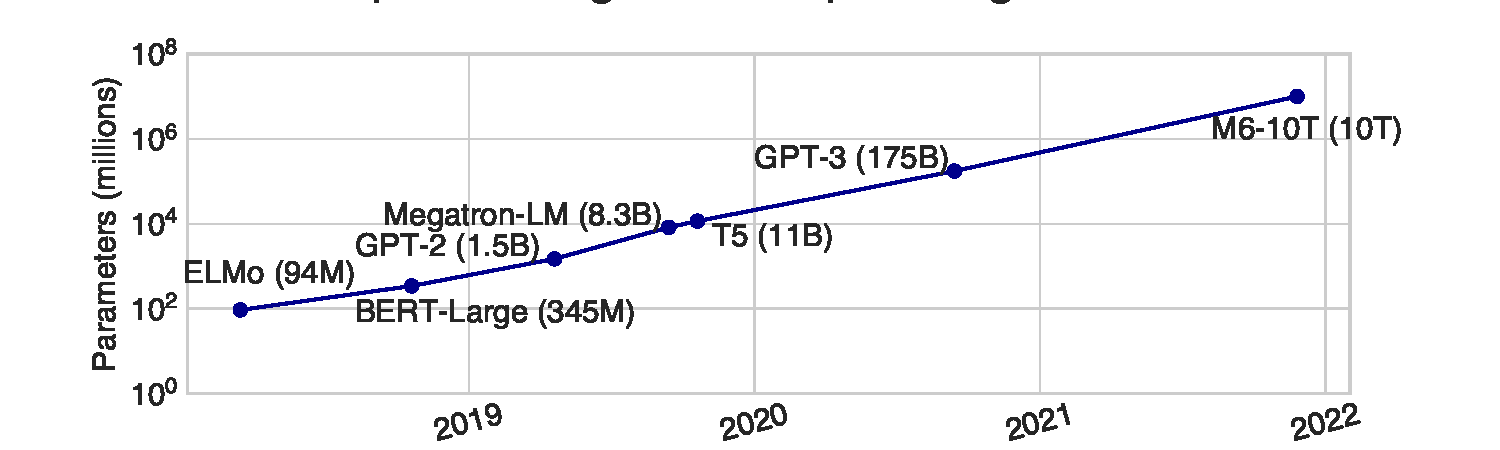
\includegraphics[keepaspectratio=true, width=\linewidth]{images/scaling_over_time}
	\caption{Illustration of how state-of-the-art DL Transformer models have grown over time.}
	\label{fig:scaling}
\end{figure}

Recent developments in DL practice have introduced a pressing new challenge of \textit{model scale} in systems for DL research. Practitioners
have begun to explore the use of very large neural architecture graphs for DL models, with some containing billions and 
even \textit{trillions} of trainable parameters! Key examples include the NLP Transformer models BERT-Large~\cite{bert2018}, GPT-3~\cite{gpt2020}
and Meta's deep learning recommender model (DLRM)~\cite{dlrm2019}. The sheer size of these models has introduced critical challenges in three key areas.

\begin{enumerate}
\item \textbf{Memory Scalability.} Standard DL training typically holds a model's parameters on the memory of an accelerator (e.g. GPU) and uses sampled data to compute gradient updates for each parameter. For a very large model, the space required to hold the parameters, intermediate computations, and gradient updates will typically exceed the relatively limited memory of an accelerator. High-end consumer-grade GPUs such as the Tesla V100~\cite{teslav100} have 16-32GB of on-device memory, but a large-scale DLRM might require hundreds of gigabytes of space.
\item \textbf{Performance.} Increased parameter counts are typically (but not always) correlated with higher execution times. Training a more complex model architecture can also require more data --- GPT-3 was trained on 300B tokens, for example~\cite{gpt2020} and the open-source BLOOM language model was trained on 366B~\cite{bloom2022}. Training such models can require weeks, or even months~\cite{dlrm2019,bloom2022}. As such, optimizations that can improve execution performance are highly beneficial
for developers of large-scale DL models.
\item \textbf{Cost of Training.} Standard solutions to the previous two challenges typically involve parallelizing storage or execution across multiple accelerators. However, this approach can drive up compute costs significantly. BLOOM was trained on 416 A100 GPUs, and Megatron-LM used 512~\cite{megatronlmblog2020}. This is not practical for most practitioners, particularly when these GPUs need to be reserved for a training period of weeks or even months. Reproducing BLOOM's training procedure on AWS
would cost 5.5 million dollars. Note that this does not even account for the added costs of model selection, wherein multiple models are trained to evaluate the best hyperparameter settings and configurations.
\end{enumerate}

As practitioners continue to push the bounds of model scale, it becomes increasingly necessary that these challenges are addressed to enable further development in the large-model DL space. As a result, various systems and techniques have been developed tackling one or another of these problems. Some directions include data spilling/CPU offloading
~\cite{zero2019, zero2021,hydra2021,mpms2021,swapadvisor2021,l2l2020}, pipeline/model parallelism~\cite{gpipe2018,pipedream2018,terapipe2021,torchgpipe2020,megatronlmgpuscaling2021}, rematerialization~\cite{checkpointing2016}, and hybrid parallelism~\cite{flexflow2018,alpa2022,hydra2021,mpms2021,gshard2020}. These subjects, falling under the general umbrella of ``large-model training techniques'', has become a key focus for researchers across industry and academia, but the sheer volume of work in the space has made this topic difficult to navigate. This paper will provide a comprehensive review of the current state of the large-model DL training systems space, along with an assessment of future directions of growth and development in the area.

A few high-level surveys on the area have recently been released~\cite{surveylarge2022,lowmemory2019} but they are not comprehensive, and do not address key topics such as model selection, hybrid parallelism, and serverless execution. This paper will address these areas and also go into further depth on state-of-the-art techniques.

Note that this survey will not cover \textit{graph neural network} training as that class of architectures encounters substantially different problems from other DL models, and would require an entirely separate survey to explore in-depth~\cite{gnnsurvey2021}. It will also not cover ``model reduction'' techniques (e.g. model distillation) as these fall outside of the scope of training and go into model modification.

This paper is organized as follows: Section~\ref{sec:background} goes over some necessary background and terminology. Section~\ref{sec:large_model} describes large-model architectures and some key examples. Section~\ref{sec:mlsys} explores the landscape of large-model DL training systems. Finally, Section~\ref{sec:conclusion} concludes the survey and explores possible future directions and emerging challenges. .




